\section{Netze}
	\subsection{Komponenten und Technologie von Stromnetzen}
		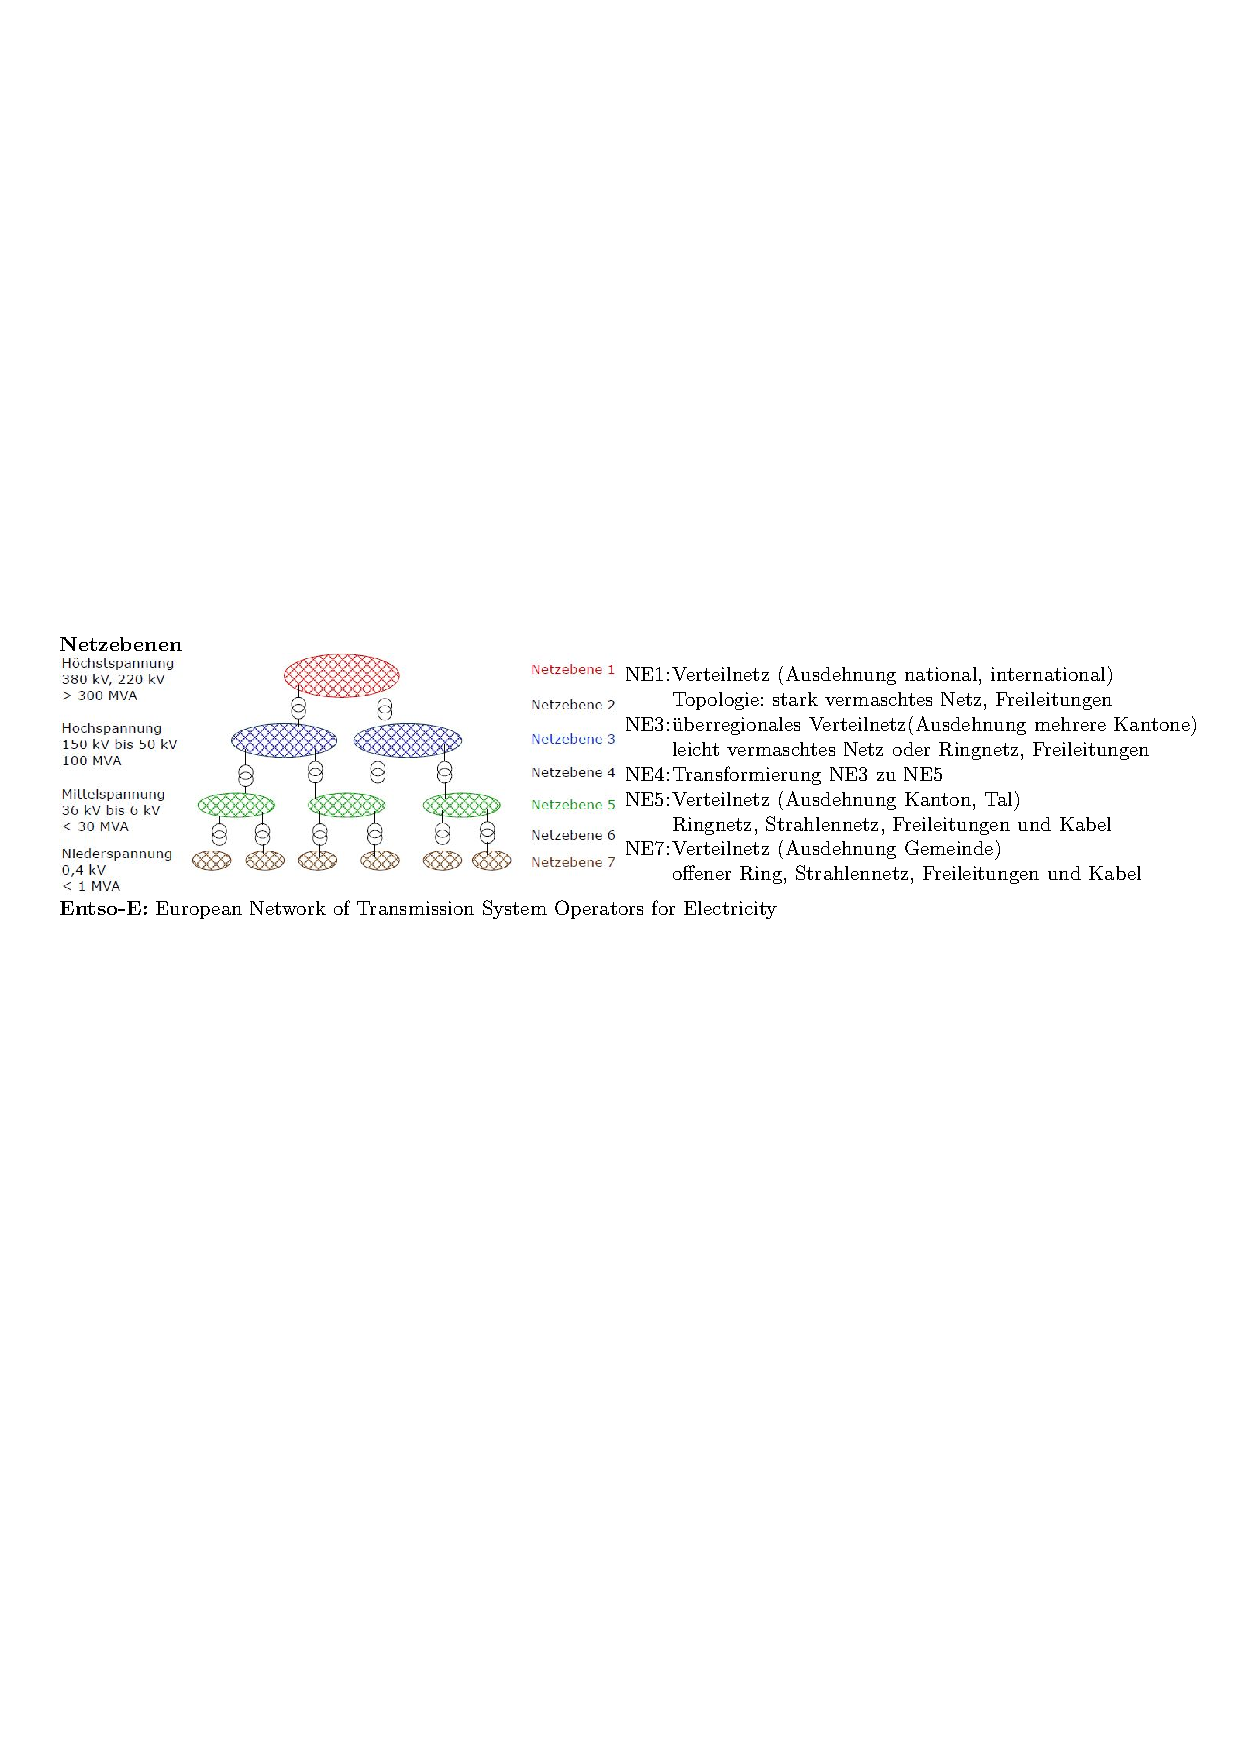
\includegraphics[width=\textwidth]{./images/Netztopologie.pdf}
		
	\subsection{Leitungsbeläge}
	\begin{multicols}{2}
		\textbf{Widerstandsbelag}\\
		Ursache: ohmscher Widerstand des Leiters \\
		$R' = \sigma \frac{\rho}{A}$, $R'$ in $\Omega/m$ \\
		$\sigma$: Verseilfaktor $\left(\sigma \approx 1.07\right)$, $\rho$: Leitungsfähigkeit in $\Omega mm^2/m$, \\
		$A$: Leiterquerschnitt in $mm^2$, $k_{SR}$: Skineffekt \\
		
		\textbf{Induktivitätsbelag}\\
		Ursache: Verkettung der magnetischen Flüsse \\
		$L' = 2 \cdot 10^{-7} \cdot \left(\ln \frac{d}{r_{eq}} + \frac{1}{4}\right) \hspace{1cm} d = \sqrt[3]{d_{12}d_{23}d_{31}}$ \\
		$r$: Leiterradius in $m$, $d$: mittlerer Leiterabstand in $m$ \\
		$d_{ij}$: Abstand zwischen Phase $i$ und $j$ \\
		
		\textbf{Ableitbelag} \\
		Ursache: Korona- und Kriechstromverluste an der Oberfläche\\
		$G'$ in $S/m \Rightarrow$ kann in vielen Fällen vernachlässigt werden\\ \\
		
		\textbf{Kapazitätsbelag}\\
		Überlagerung der Einzelspannungen liefert den Kapazitätsbelag $C'$ in $F/m$ \\
		$C' = \frac{2\pi \epsilon}{\ln \frac{d}{r_{eq}}}$\\
		$r$: Leirerradius in $m$ \\
		$d$: mittlerer Leiterabstand in $m$ \\ 
	\end{multicols}
	\textbf{Bündelleiter}\\
		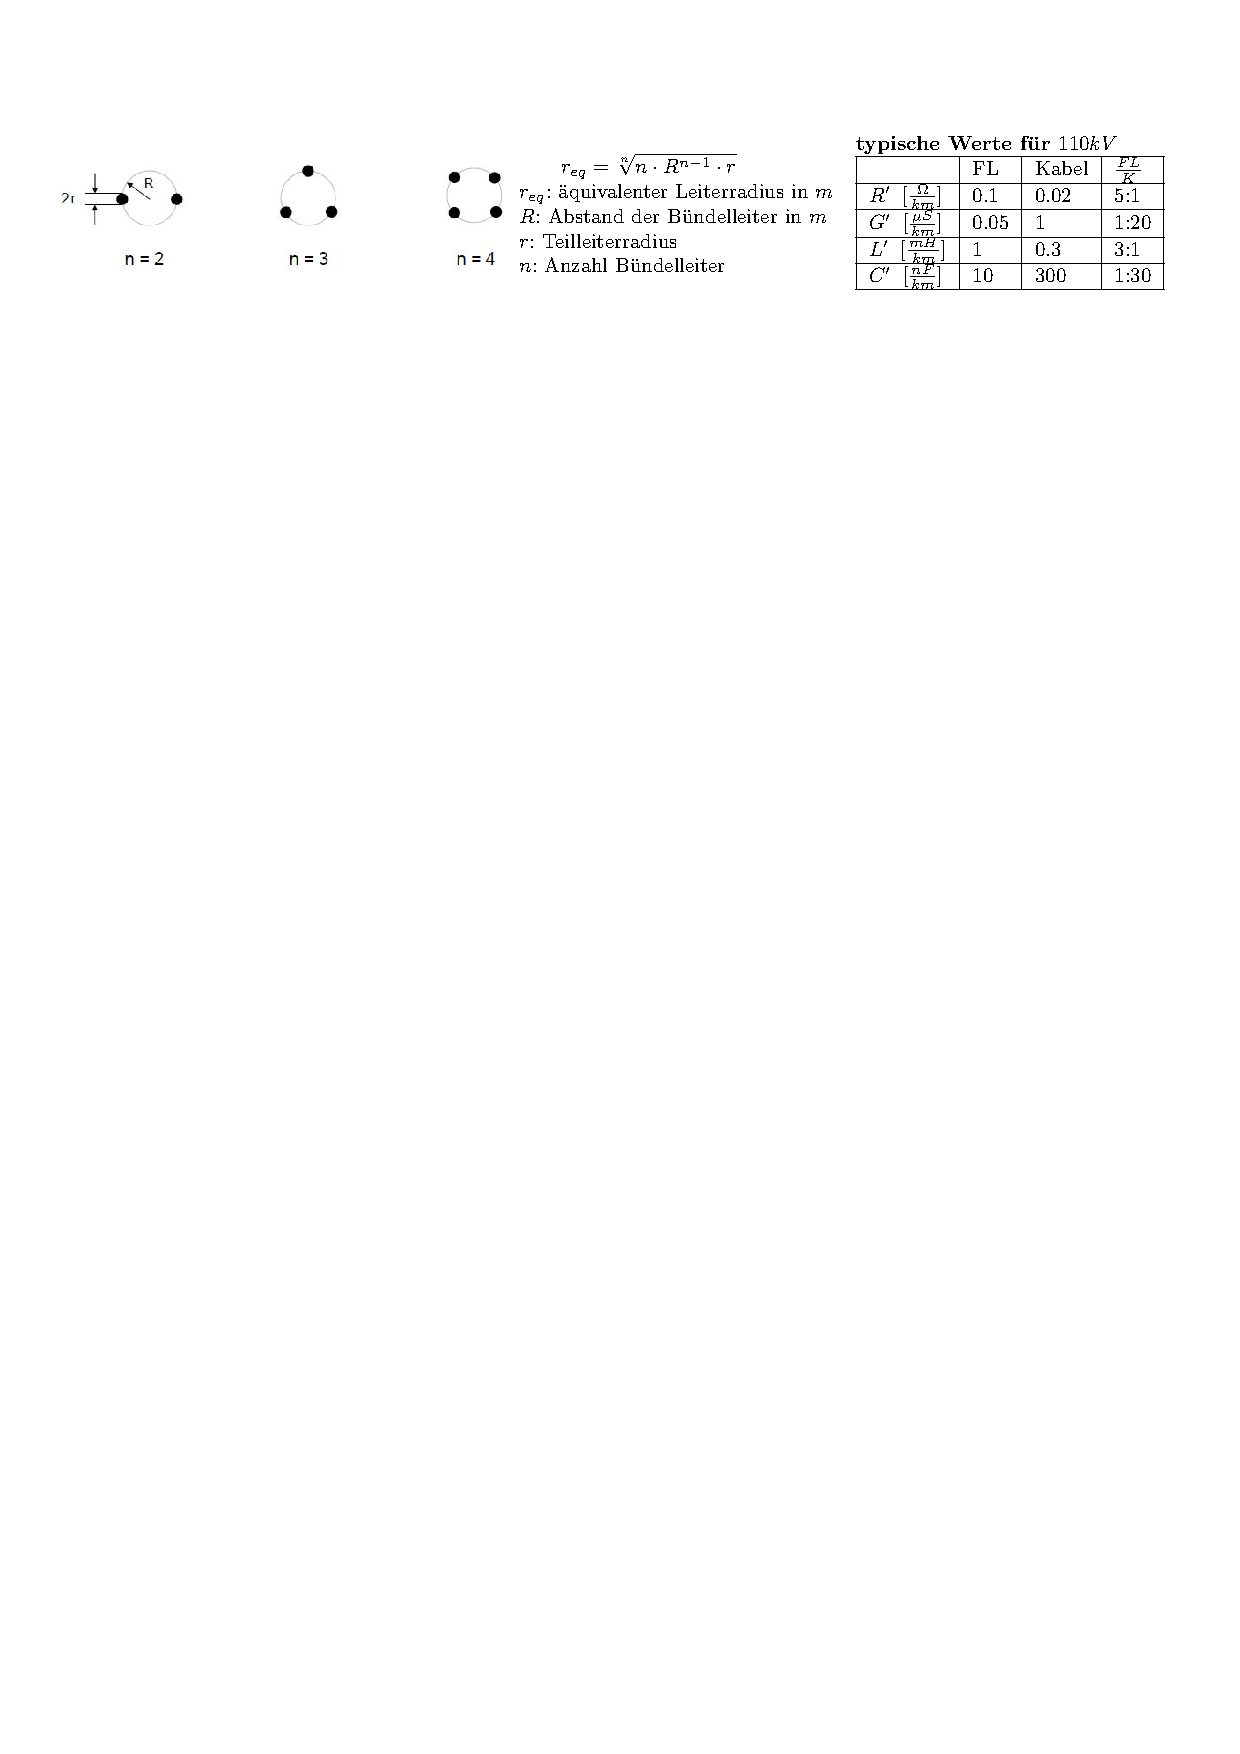
\includegraphics[width=\textwidth]{./images/Buendel.pdf}
	\begin{multicols}{2}
		\textbf{Sag} \\
		\begin{minipage}[lt]{5cm}
			\centering
			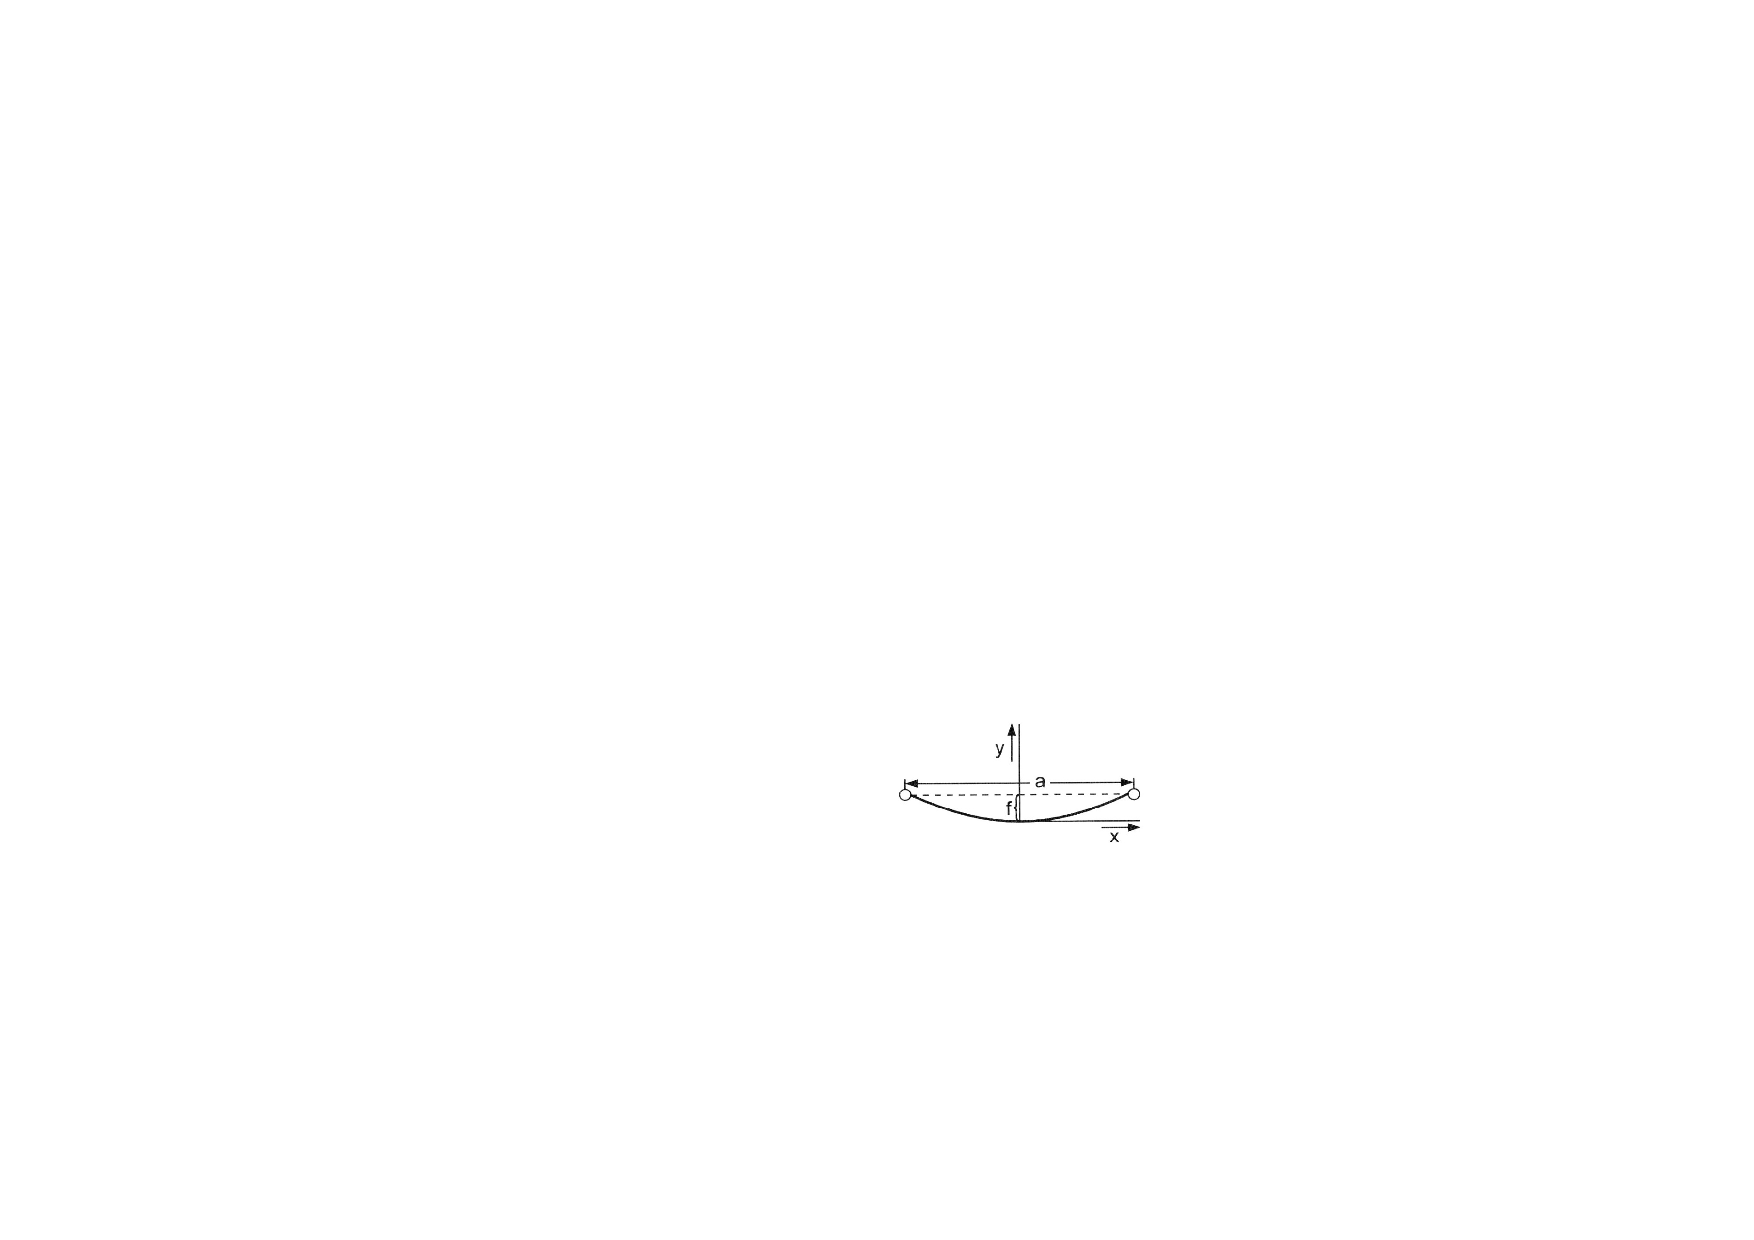
\includegraphics[width=0.7\textwidth]{./images/sag.pdf}
		\end{minipage}
		\begin{minipage}[rt]{5cm}
			$y \approx \frac{mg}{2\sigma}x^2$ \\
			$f_{max} = y \cdot \left(a/2\right)^2$ \\
			$h_{min} = 6 + \frac{U_N - 110~kV}{150~kV}$ 
		\end{minipage}

		\textbf{Skin effect}\\
		{\small $R_\sim = R_= \cdot k_s; \hspace{1cm} k_s \approx 1 + \frac{1}{3}\eta^4$\\
		$ \eta = \frac{r}{2\delta}; \hspace{1cm} \delta = \sqrt{\frac{2\rho}{\omega \cdot \mu}}$ \\
		$R_= = \frac{\rho(\vartheta)\cdot l}{A}; \hspace{1cm} \rho(\vartheta) = \rho_{20} [1+\alpha\left(\vartheta - 20^\circ C\right)]$\\}
	\end{multicols}
		
		
	\subsection{Leitungsmodell und Betriebsverhalten}
		\begin{multicols}{3}
			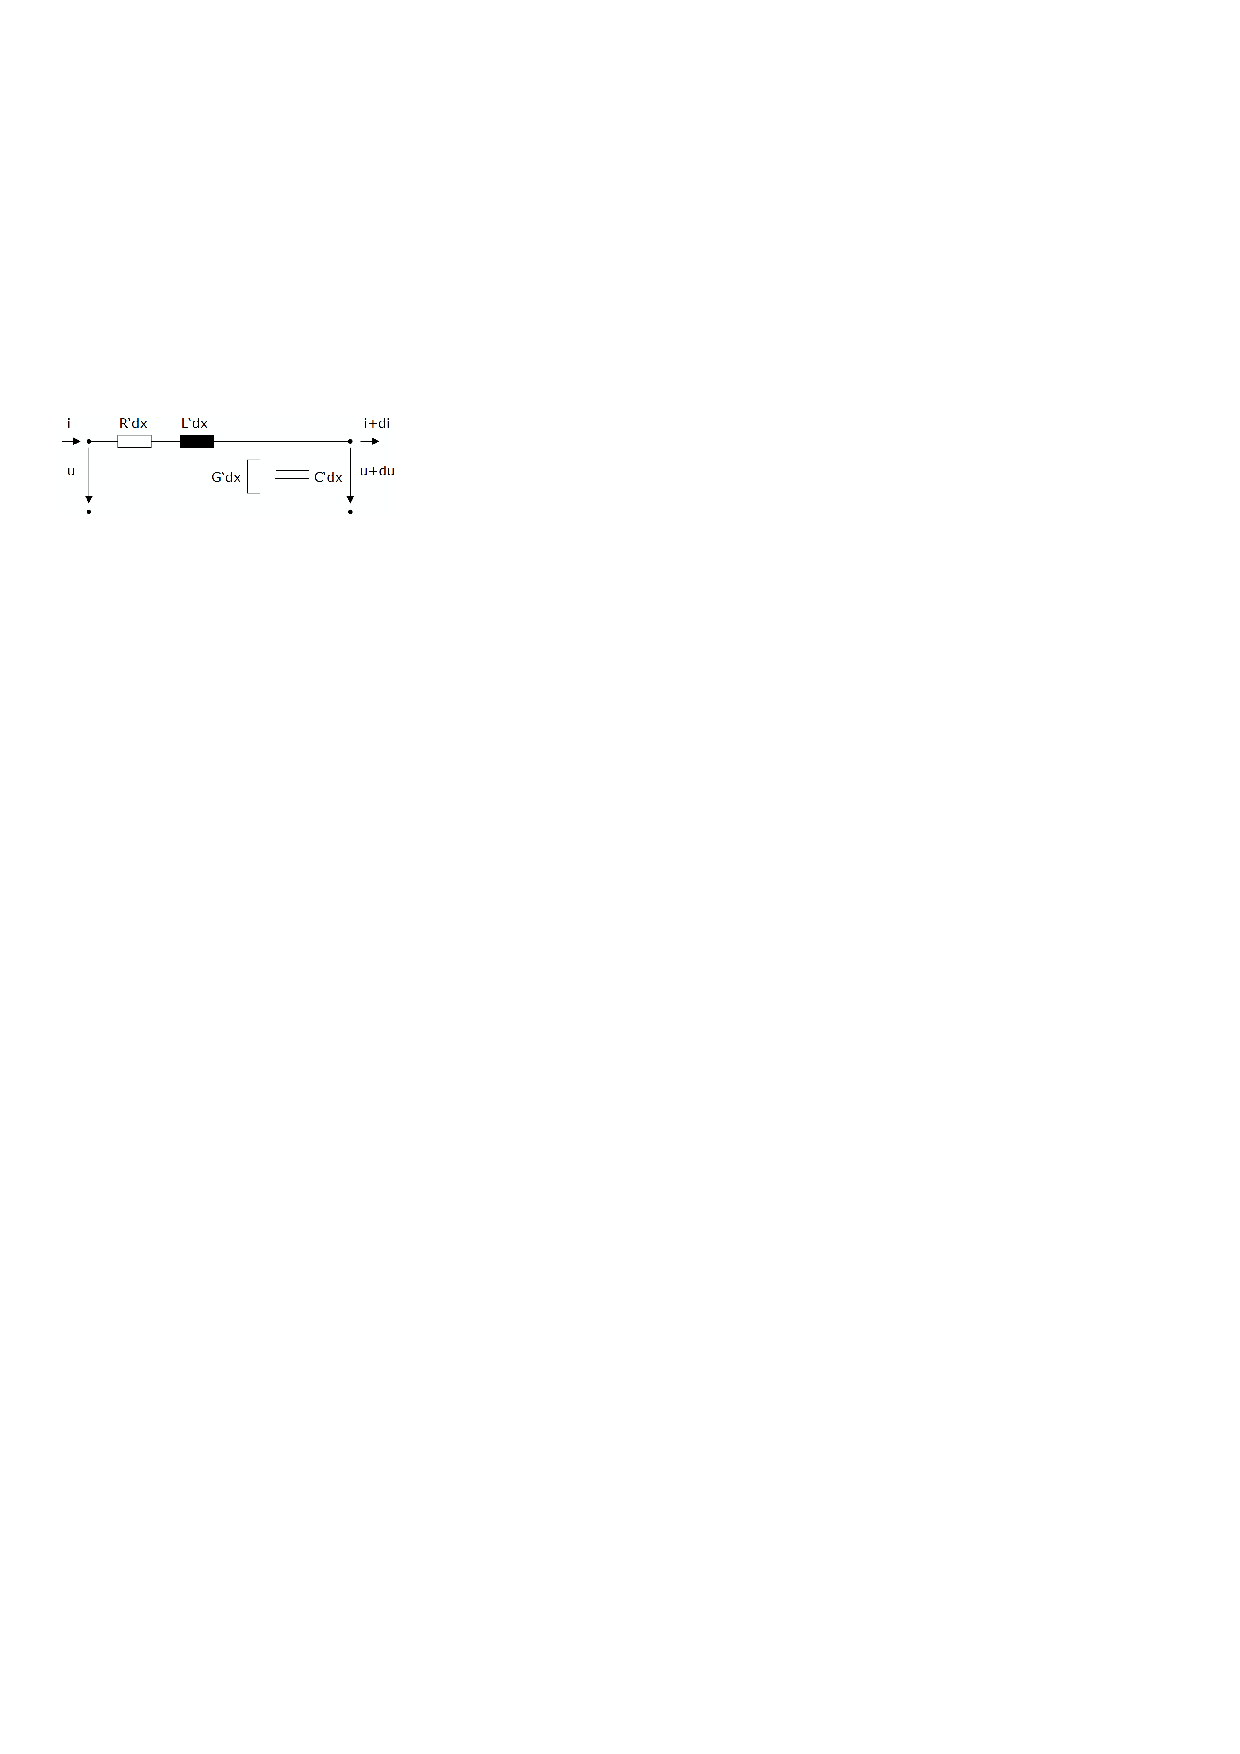
\includegraphics[width=0.28\textwidth]{./images/Leitungsmodell1.pdf} 
			
			allgmeine DGL: \\
			$-du = R'dx \cdot i + L'dx \cdot \frac{di}{dt}$\\
			$-di = G'dx \cdot u + C'dx \cdot \frac{du}{dt}$ \\
			
			DGL für Wechselstrom:\\
			$\frac{d\underline{U}}{dx} = R'\underline{I} + j \omega L' \underline{I}$ \\
			$\frac{d\underline{I}}{dx} = G'\underline{U} + j \omega C' \underline{U}$ 
		\end{multicols}
		Lösung für Wechselstrom:\\
		$\underline{U}_1 = \underline{U}_2 \cosh \underline{\gamma}l + \underline{Z}_w \underline{I}_2 \sinh \underline{\gamma}l \hspace{0.8 cm} \underline{I}_1 = \frac{\underline{U}_2}{\underline{Z}_w} \sinh \underline{\gamma}l + \underline{I}_2 \cosh \underline{\gamma}l \hspace{0.8cm} \underline{\gamma} = \sqrt{\left(R' + j \omega L'\right) \left(G' + j \omega C'\right)}~[\frac{1}{m}] \hspace{0.8cm} \underline{Z}_w = \sqrt{\frac{R' + j\omega L'}{G' + j \omega C'}}~[\Omega]$ \\
		$Z_w \approx \sqrt{X_L X_C} = \frac{1}{2\pi} \sqrt{\frac{\mu_0}{\epsilon_0}} \ln \frac{d}{r} \hspace{1cm}$ \\
		
		\textbf{PI-Ersatzbild (vereinfacht)} \\
		\begin{minipage}[lt]{6cm}
			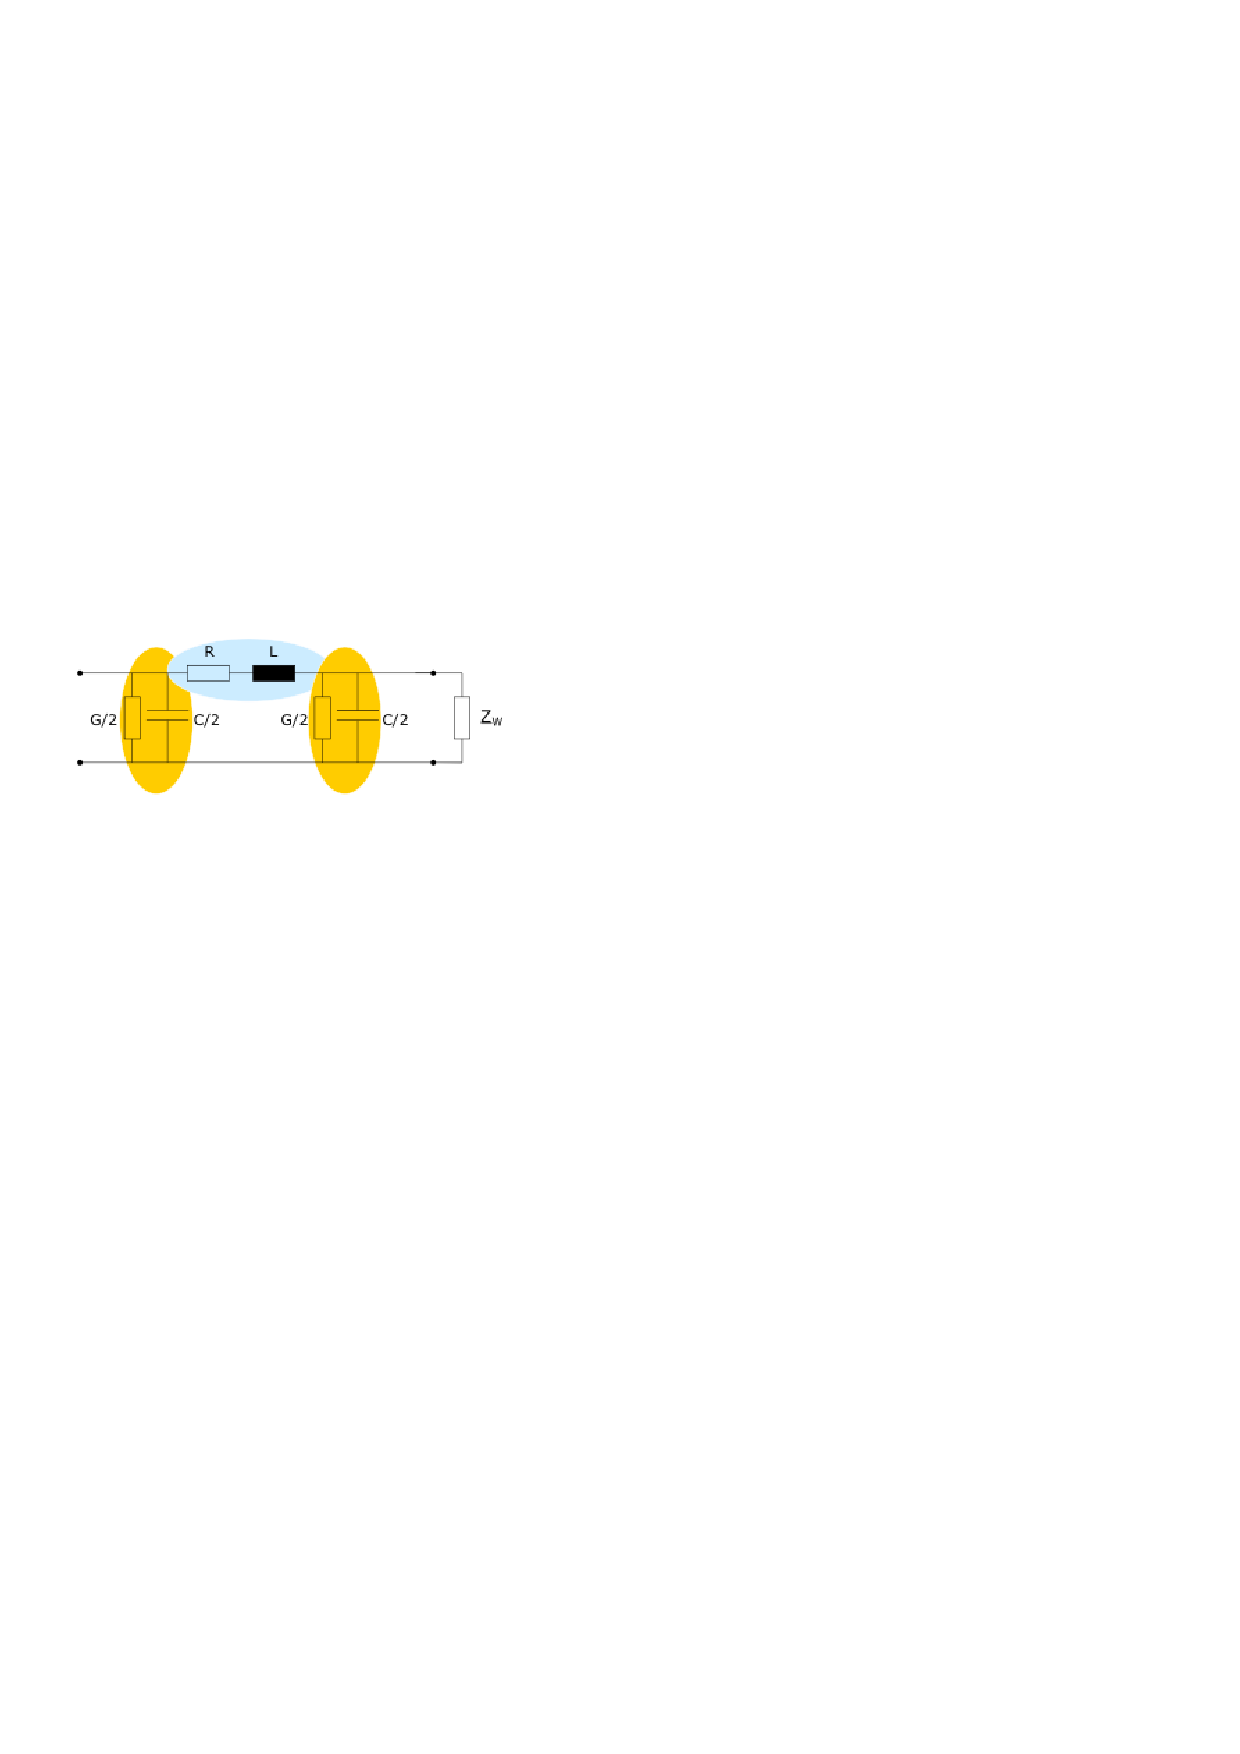
\includegraphics[width=0.9\textwidth]{./images/Leitungsmodell2.pdf}
		\end{minipage}
		\begin{minipage}[rt]{13cm}
			Vereinfachte Modellierung einer Leitung, jedoch nur wenn kürzer als $250~km$(FL)/$50~km$(Kabel) und die Frequenz $50~Hz$ ist. Ersatzbild mit Querimpedanz (gelb) und Längsimpedanz (blau).
		\end{minipage}
		\textbf{Erwärmung der Isolation}: $\tan \delta = \frac{G}{\omega C} \Rightarrow P_V = 3 \cdot U^2 G = U^2 \omega C \cdot \tan \delta$ \\
		\textbf{Spannungsabfall (vereinfacht)}: $\Delta U = \frac{P \cdot R}{U_N} + \frac{Q \cdot X}{U_N}; \hspace{1cm} \Delta u = \frac{\Delta U}{U_N}; \hspace{1cm}$ messen: $\Delta u = \frac{S_A \cdot \cos \varphi}{S_K} \hspace{1cm} \Delta U \approx  \Delta U_L = \sqrt{3} \cdot I \cdot X_L$\\
		\textbf{Relativer Spannungsabfall}: $d = \frac{\Delta U}{U_V} \approx \frac{\Delta S_A}{S_K} \cdot cos(\psi_{K} - \phi) \hspace{1cm}\psi:$ network impedance angle, $\varphi:$ angle of load ($\approx 60^\circ$)\\
		\textbf{Verluste in Leitung}: $P_V = 3 \cdot I^2 \cdot R \hspace{1cm} Q_{ind} = 3 \cdot I^2 \cdot X_L \hspace{1cm} Q_{cap} = \frac{U^2}{X_C} \hspace{1cm} Q_{ges} = Q_{ind} - Q_{cap}$ \\
		\textbf{Ferranti-Effekt}: $\underline{U}_1 = \underline{U}_2 + jX_L \cdot \underline{I}_2; \hspace{1cm} \underline{I}_2 = \frac{\underline{U}_E}{-2jX_C}; \hspace{1cm} \Rightarrow \frac{U_2}{U_1} = \left(1 - \frac{X_L}{2X_C}\right)^{-1} \hspace{1cm} \Delta U = \frac{1}{2} U_1 \omega^2 l^2 C' L'$\\
		
	\subsection{Begriffe}
		\begin{itemize}
				{\small \setlength{\itemsep}{0pt}
				\item \textbf{Kurzschluss}: extreme übernatürliche Belastung, Leitung verhält sich wie $L$, Spannung sinkt entlang der Leitung ab.
				\item \textbf{Leerlauf}: extreme unternatürliche Belastung, Leitung verhält sich wie $C$, $U$-Überhöhung am Leitungsende, Ferranti-Effekt
				\item \textbf{Natürliche Leistung}: Bei einer gewissen Belastung wird in den Querelementen genau so viel Blindleistung erzeugt, wie im Längspfad verbraucht wird. Die Leitung verhält sich neutral bezüglich Blindleistung. Die natürliche Leistung wird übertragen, wenn die Leitung mit $\underline{Z}_w$ belastet wird. $\hspace{1cm} \underline{I}_2 = \frac{\underline{U}_2}{\underline{Z}_w}; \hspace{1cm} \underline{U}_1 = \underline{U}_2 \left(\cosh \underline{\gamma} l + \sinh \underline{\gamma}l\right) = \underline{U}_2e^{\underline{\gamma}l}; \hspace{1cm} I_{nat} = \sqrt{\frac{U_N^2}{3X_LX_C}} = \sqrt{\frac{U_N^2}{3L'/C'}}$
				\item \textbf{Übernat. Belastung}: $\underline{Z}_{Last} < \underline{Z}_w, \underline{Q}_{quer} < \underline{Q}_{laengs}, U$ an Leitungsende ist tiefer als $U$ am Leitungsanfang (KS)
				\item \textbf{Unternat. Belastung}: $\underline{Z}_{Last} > \underline{Z}_w, \underline{Q}_quer > \underline{Q}_{laengs}, U$ an Leitungsende ist höher als $U$ am Leitungsanfang. Freileitungen werden meistens, Kabel immer unternatürlich betrieben (Leerlauf, kapazitiv)
				\item \textbf{Wellenimpedanz}: typische Werte: Freileitungen $\lvert \underline{Z}_w \rvert \approx 300~\Omega$, Kabel $\lvert \underline{Z}_w \rvert \approx 40~\Omega$
				}
		\end{itemize}	
	\subsection{Transformatormodell}
		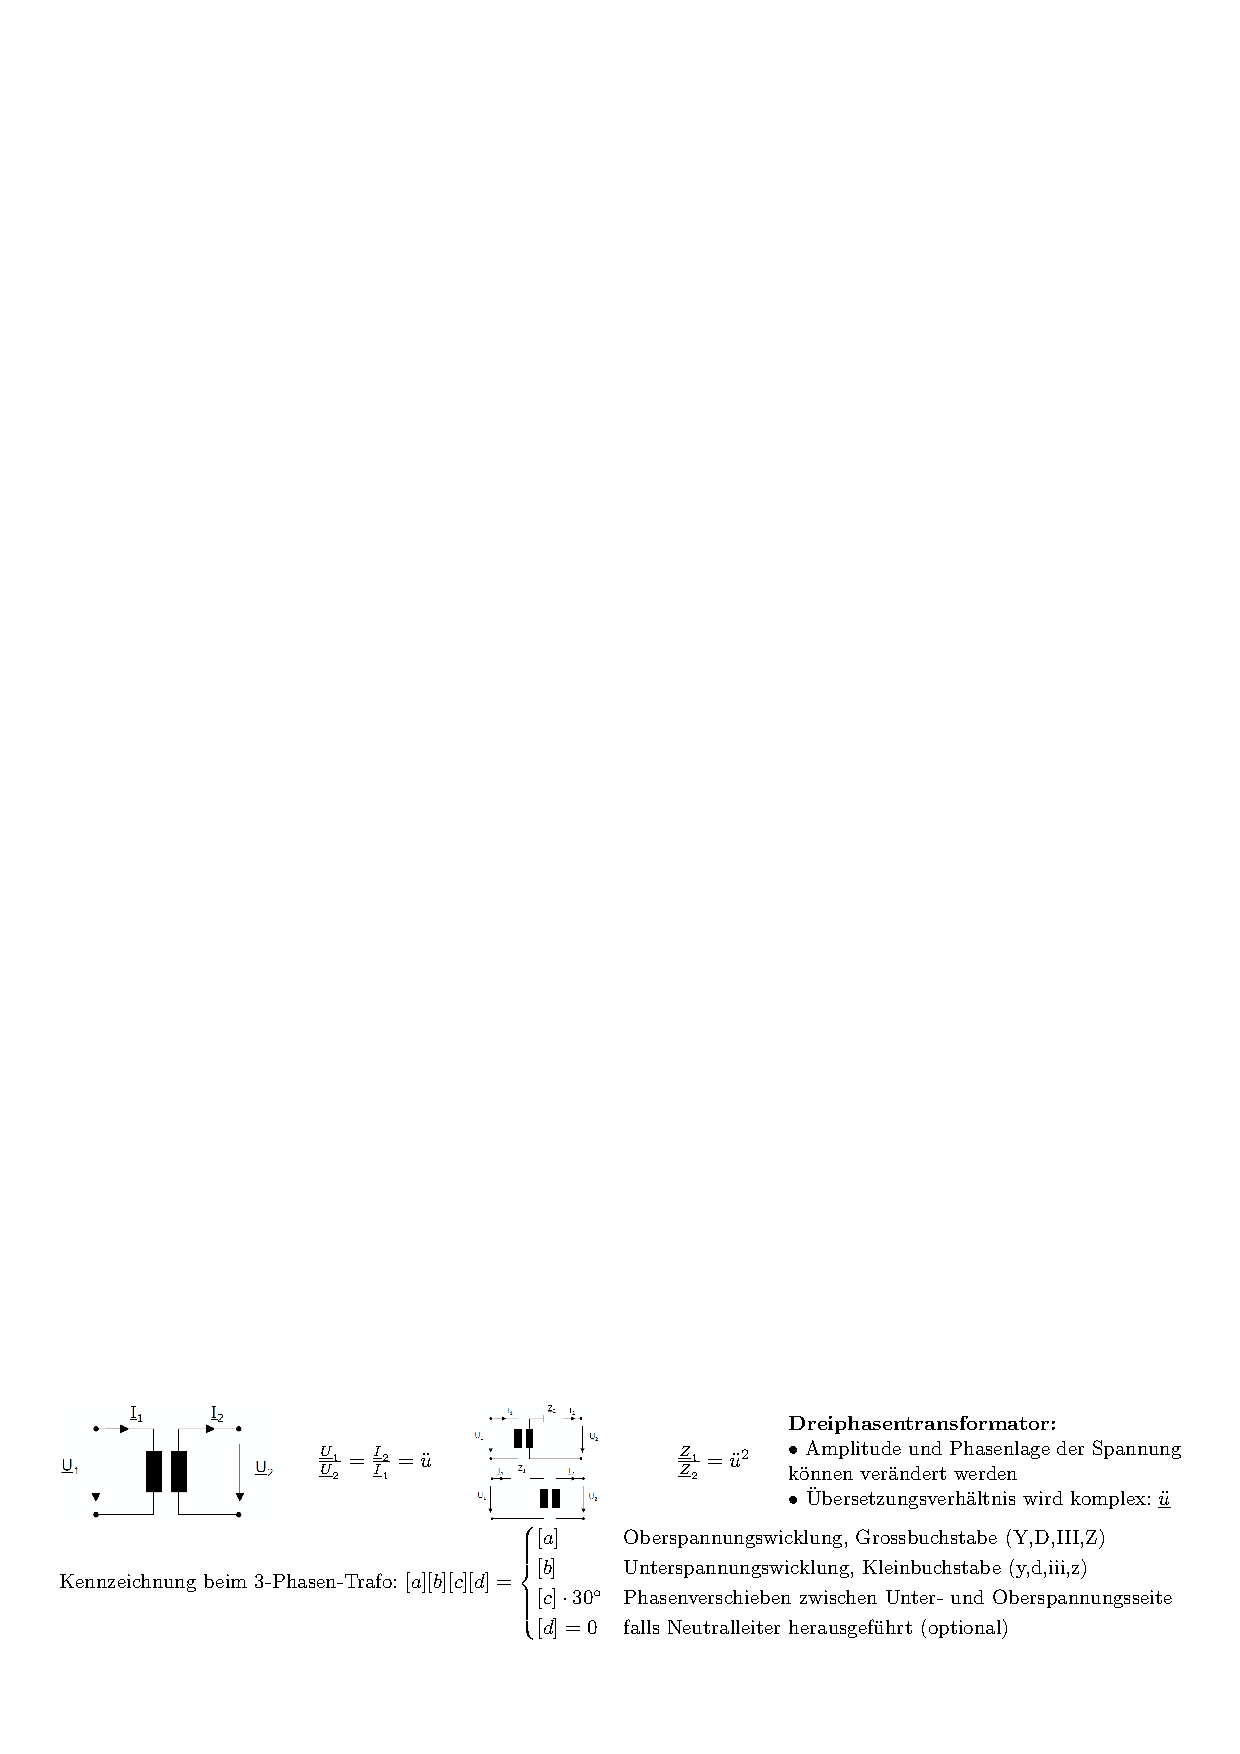
\includegraphics[width=\textwidth]{./images/Trafomodell.pdf}
		ü$_0 = \frac{w_1 \pm \Delta w_1}{w_2} = $ü$_N + \Delta$ü \\
		$X_T = u_K \cdot \frac{U_N^2}{S_{NT}}$
	\subsection{Active power transmission}
		\includegraphics[width=\textwidth]{./images/MOdellierung.pdf}	
		
	\subsection{Frequenzregelung im Verbundnetz}
		grid droop for UCTE: $c_P = \frac{\Delta P / P_N}{\Delta f / f_N}  \approx 0.5; \hspace{1cm}$ Droop: $s = - \frac{\Delta f / f_N}{\Delta P / P_N}; \hspace{1cm}  K_{Regulation} = \frac{\Delta P}{\Delta f} = s^{-1} \frac{P_N}{f_N} \quad [MW/Hz]$ \newline
		
		\textbf{Primärregelung - erste Sekunden (15- 30 s): alle reagieren}\newline
		$\bullet$ dezentrale Regelung  $\bullet$ basiert auf lokaler Frequenzmessung  $\bullet$ Frequenz-Leistungs-Statistik = P-Regler (bleibende Abweichung!)  $\bullet$ findet vollautomatisch und lokal im Turbinenregler des Kraftwerks statt  $\bullet$ Erbringung im gesamten Netzgebiet  $\bullet$ gesamte Netzkennzahl $MW/Hz$ wird auf Länder aufgeteilt  $\bullet$ jedes Land leistet entsprechenden Beitrag (CH $\approx 70~MW$, UCTE $\approx 3000~MW/Hz$)  $\bullet P_P = \Delta f \cdot K_{CH}$ \newline
	
		\textbf{Sekundärregelung - erst Minuten: ausgewählte 'Teamkollegen' übernehmen}\newline
		$\bullet$ basiert auf Messwertsummen der Grenzleitungen, Frequenzabweichungen und dem Korrektursignal Synchronzeit  $\bullet$ PI-Regler  $\bullet$ führt Frequenz zurück auf Sollwert $f_{soll} = f_{old} + \frac{\Delta P_{SR}}{K_{SR}}$  $\bullet$ findet vollautomatisch im zentralen Netzregler der Regelzone statt  $\bullet$ Erbringung durch entsprechende Regelzone  $\bullet$ CH $\approx 400~MW$ \newline
		
		\textbf{Tertiärregelung - nach einigen Minuten: 'Ersatzfahrer' steigt auf}\newline
		
		$\bullet$ Entlastung der Sekundärregelung  $\bullet$ zentral und manuell durchgeführt  $\bullet$ manueller Abruf  $\bullet$ ermöglicht nach einer Störung die neuerliche Optimierung des Kraftwerkeinsatzes  $\bullet$ Dispatcher trifft Entscheidungen  $\bullet P_T = P_{Ausfall} - P_P - P_S$  $\bullet$ CH $\approx +450/-390~MW$ 
		
		
	\subsection{Netzsicherheit und Massnahmen}
	\begin{minipage}[lt]{14cm}
		\textbf{$n-1$-Sicherheit}\newline
		$\bullet$ der Ausfall eines Betriebsmittels darf zu keiner Überlastung eines anderen Betriebsmittels führen  $\bullet$ $n$: ist die aktuelle Anzahl der Betriebsmittel  $\bullet$ nach Ausfall eines Betriebsmittels stehen nur noch $n-1$ Betriebsmittel zu Verfügung  $\bullet$ bei Verletzung der $n-1$-Sicherheit ist noch nichts passiert  $\bullet$ keine $n-1$-Sicherheit = keine Reserve  $\bullet$ Verhinderung Kaskadeneffekt \newline
		
		\textbf{Massnahmen bei Gefährdung der Netzsicherheit} \newline
		$\bullet$ Topologische Massnahmen (Umleiten der Lastflüsse durch Veränderung der Topologie $\Rightarrow$ Änderung der Sammelschienen Konfiguration, Stufen von Transformatoren, Zu-/Abschalten von Leitungen und Trafos, FACTS)  $\bullet$ Produktionsverschiebung (Redispatch $\Rightarrow$ Eingriff in die Produktion = Eingriff in den Markt = unerwünscht)  $\bullet$ Lastabwurf (siehe Abb. \ref{Grid:freq})
	\end{minipage}
	\begin{minipage}[rt]{5cm}
		\hfill
		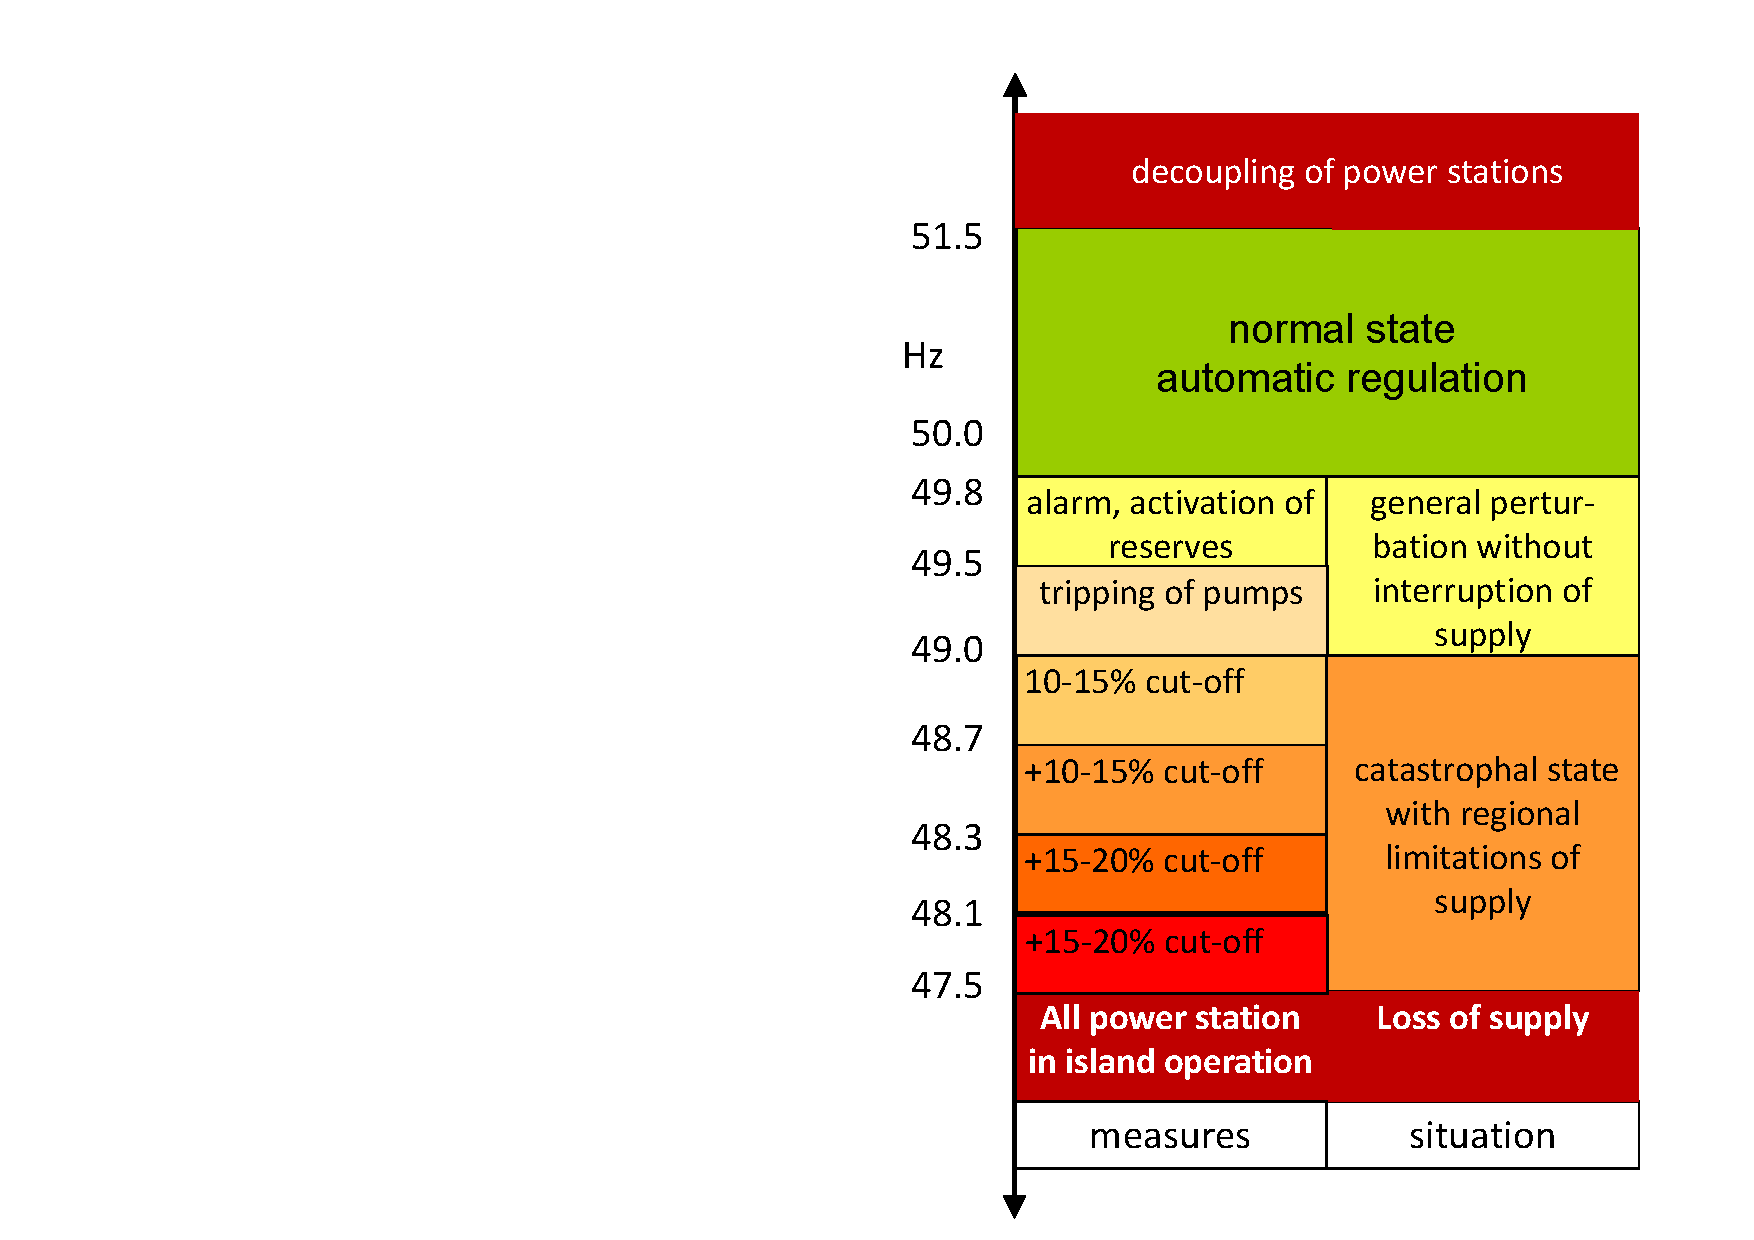
\includegraphics[width=0.75\textwidth]{./images/frequenz.pdf}
		\label{Grid:freq}		
	\end{minipage}
	
	\subsection{Voltage quality}
	\begin{multicols}{2}


		{\footnotesize 	\begin{itemize}
		\setlength{\itemsep}{0pt}
		\item \textbf{voltage}: sinusoidal as possible, amplitude and frequency in rated values
		\item \textbf{harmonics}: reduced durability of capacitors and motors \\$\rightarrow THD_u = \frac{\sqrt{\sum_{i = 2}^{40} U_i^2}}{U_1} \leq 8 \% \hspace{1cm} THD_i = \frac{\sqrt{\sum_{x = 2}^{50} I_x^2}}{I_A} \leq \frac{20}{1000} \cdot \sqrt{\frac{S_{K}}{S_A}}  $
		\item \textbf{flickere (periodic voltage oscillation)}: oscillation of the light density
		\item \textbf{unbalance}: thermal losses/vibrations in el. machines
		\item \textbf{(commutation-)notches}: disturbance of process controls, crash
		\end{itemize}}
	
		{\footnotesize 	\begin{tabular}{|c|c|c|c|}
		\hline \textbf{Characteristic of} &\textbf{Values/} & \textbf{mean} & \textbf{observation}\\
		 \textbf{the voltage} & \textbf{tolerance} & x & \textbf{time} \\ 
		\hline \textbf{Frequency} & $50~Hz; \pm 1\%$ & 10 s & 1 year \\ 
		\hline \textbf{Voltage magnitude} & $\pm 10\% U_N$ & 10 min & 1 week \\ 
		\hline \textbf{longterm flicker} & $P_{lt} = 1$ & 2h & 1 week \\ 
		\hline \textbf{Harmonics} & $THD \leq 8\%$ & 10 min & 1 week \\ 
		\hline \textbf{Unbalance} & $U_2/U_1 < 2\%$ & 10 min & 1 week \\ 
		\hline 
		\end{tabular} }
	\end{multicols}
	
	\subsection{HVDC}
	\begin{minipage}[lt]{13cm}
		{\footnotesize 	\begin{tabular}{|c|c|c|c|}
		\hline  & \textbf{HVAC} & \textbf{HVDC} & \textbf{HVDC/HVAC} \\ 
		\hline Nominal voltage for & $U_\lambda = \frac{U_{Iso}}{\sqrt{2}}$ & $U_{DC} = U_{Iso}$& $\frac{U_{DC}}{U_{AC}} = \frac{\sqrt{2}}{\sqrt{3}}$\\
		the same isolation & $\Rightarrow U_{AC} = \frac{\sqrt{3}}{\sqrt{2}} \cdot U_{Iso}$ & 
		 &  \\ 
		\hline Transmission power & $S_{AC} = \sqrt{3} \cdot U_{AC} \cdot I_{AC}$ & $S_{DC} = 2 \cdot U_{DC} \cdot I_{DC}$ & $\frac{2 \sqrt{2} \cdot I_{DC}}{3 \cdot I_{AC}}$ \\ 
		\hline Transmission losses & $P_{VAC} = 3 \cdot I_{AC}^2 \cdot R_{AC}$ & $P_{VDC} = 2 \cdot R_{DC} \cdot I_{DC}^2$ & $\frac{9 \cdot R_{DC}}{3 \cdot 4\cdot R_{AC}} \approx \frac{3}{4}$ \\ 
		\hline Material (ropes) & $V_{AC} = 3 \cdot A_{AC} \cdot l$ & $V_{DC} = 2 \cdot A_{DC} \cdot l = \frac{3}{2} \cdot A_{AC} \cdot l$ & 0.5 \\ 
		\hline 
		\end{tabular} }
	\end{minipage}
	\begin{minipage}[rt] {6cm}
		$U_{DC \alpha} = 1.35 \cdot U_\Delta \cdot \cos \alpha$ \\
		$\alpha:$ firing angle\\
		$U_{DC} = \frac{1}{\pi/3} \int_{-\pi/6}^{\pi/6} \sqrt{2}U \cos(\omega t) d(\omega t)$\\
		Converter: $U_{AC\Delta} = \frac{U_{DC}}{1.4 \cdot 2}$\\
		$D_{w\Delta Y} = \frac{U_1 \cdot \sqrt{3}}{U_2} \hspace{1cm} D_{w\Delta\Delta} = \frac{U_1}{U_2}$\\
		$D_{wY\Delta} = \frac{U_1}{U_2  \cdot \sqrt{3}} \hspace{1cm} D_{wYY} = \frac{U_1}{U_2}$
	\end{minipage}
	
	\begin{multicols}{2}
		\subsection{Starpoint (phase fault between $3N$)}
		\begin{itemize}
			\setlength{\itemsep}{0pt}
			\item \textbf{rigid earthing}: LV, EHV (and MV when meshed), fast identification of fault, after a longer time for all, $I_K = \frac{U_{3N}}{Z_K} = \frac{U_N/\sqrt{3}}{Z_K}$
			\item \textbf{isolated}: MV, $\underline{I}_F = \frac{\underline{U}_{13}}{-jX_{CE}} + \frac{\underline{U}_{23}}{-jX_{CE}} = \frac{\sqrt{3}U_N}{X_{CE}}$
			\item \textbf{compensated}: MV after a certain time or with enough cables, $\frac{U_{3N}}{X_D} = \frac{\sqrt{3} U_N}{X_{CE}} \Rightarrow X_D = \frac{X_{CE}}{3} \Rightarrow L = \frac{X_D}{\omega}$ 
		\end{itemize}
		
		\subsection{Short-circuit calculation}
		$I_k'' = \frac{c \cdot U_N}{\sqrt{3} \cdot Z_k}$\\
		$\underline{S}_k'' = \sqrt{3} \cdot \underline{U}_N \cdot \underline{I}_k''^*$ \\
		$\underline{Z}_k = \frac{c \cdot \underline{U}_N^2}{\underline{S}_k''^*}$\\ 
		simplified: $c = 1.1$ (siehe Tabelle \ref{tab:SM}) \\
		Single Phase Load: $S_A = k_u (\approx 0.7 \%)\cdot S_k$

	\end{multicols}